\documentclass{article}
\usepackage{pgfplots}
\title{KEEL: ROC output}
\begin{document}
\maketitle
\hfill \break
File: TEST
\hfill \break
\hfill \break
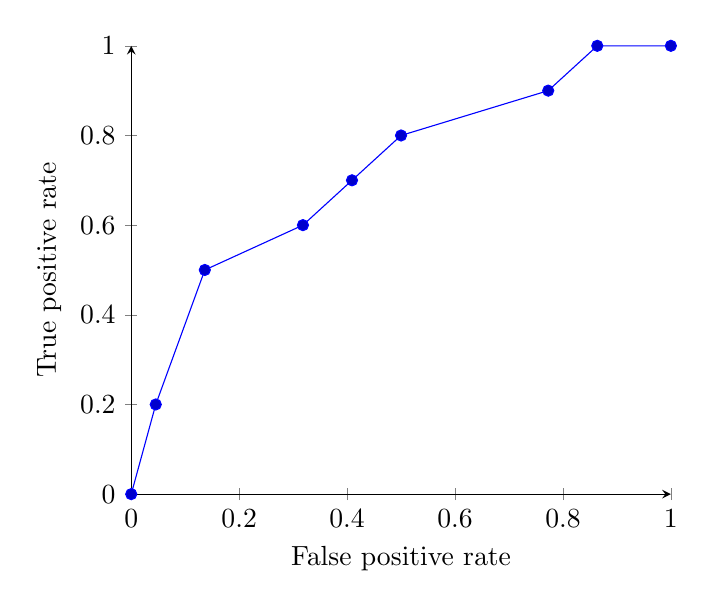
\begin{tikzpicture}
\begin{axis} [xlabel=False positive rate,
ylabel=True positive rate,axis x line=bottom,
axis y line=left]
\addplot coordinates { (0,0)(0.045454545454545456,0.2)(0.13636363636363635,0.49999999999999994)(0.31818181818181823,0.6)(0.40909090909090917,0.7000000000000001)(0.5000000000000001,0.8000000000000002)(0.7727272727272726,0.9000000000000002)(0.8636363636363634,1.0000000000000002) (1,1) };
\end{axis}
\end{tikzpicture}\hfill \break
 AUC:0.7090909090909088
\hfill \break
\end{document}